%\setcounter{section}{7}
\section{Investigating the temperature dependence of drug decomposition}
\subsection{Introduction}

During this practice we study the pseudo first-order hydrolysis reaction of acetilsalicilic acid.
The rate constant of a first-order reaction can be written as:

\begin{equation}
\label{eq:divider}
        k
        =
        \frac
                {1}
                {t}
	\ln
	\frac{z}{z-x}
\end{equation}

where $t$ is time, $z$ is the initial concentration of the reagent, $x$ is the concentration of the product at time $t$.

The reaction rate depends on temperature, which is stated in the \emph{Arrhenius law}:

\begin{equation}
\label{eq:divider}
        \frac
                {d\ln k}
                {dT}
	=
	\frac
		{E}
		{\mathrm{R}T^2}
\end{equation}

after integration:

\begin{equation}
\label{eq:divider}
        k
        =
	A
	e^{-E/( \mathrm{R} T)}
\end{equation}

and

\begin{equation}
\label{eq:divider}
        \lg k
        =
        \lg A
	-\frac{E}{2.303 \mathrm{R}T}
\end{equation}

$A$ is the preexponential factor, $E$ is the activation energy, and R is the universal gas constant (R$ = 8.314$ J/Kmol). The factor 2.303 is the conversion form ln to lg.
Activation energy can be obtained graphically if we take the slope of the function $\lg k - 1/T$ and multiply it by 2.303 $\times$ 8.314. The dimension in this case for $E$ is J/mol.
If we measure $k$ on two different temperatures ($k_1$ and $k_2$ on $T_1$ and $T_2$ temperature), activation energy can be calculated as follows:

\begin{equation}
	E
	=
	2.303
	\times
	8.314
	\lg
	\frac{k_1}{k_2}
	\frac{T_1 T_2}{T_1-T_2}
\end{equation}

\subsection{Practice procedures}

Alkaline hydrolysis of acetylsalicylic acid (Fig. \ref{fig:salicilsav}) is a pseudo first-order reaction. 
\begin{figure}
\centering
%\schemedebug{false}
%\schemestart
%	\footnotesize \chemname{\chemfig{*6(-=-(-O-[::-60]([::-60]=O)-)=(-(-[::-60]OH)=[::60]O)-=)}}{acetylsalicylic acid}
%	\footnotesize \+
%	\footnotesize \chemfig{OH^{-}}\arrow(.mid east--.mid west){->[k][]}
%	\footnotesize \chemname{\chemfig{*6(-=-(-OH)=(-([::-60]-OH)=[::60]O)-=)}}{salicylic acid} + CH$_3$COO$^-$
%\schemestop
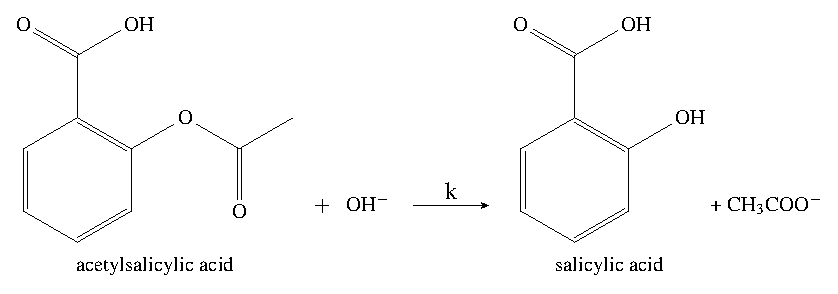
\includegraphics[width=1\textwidth]{fig/asa_hydrolysis.eps}
\caption{Alkaline hydrolysis of acetylsalicylic acid.}
\label{fig:salicilsav}
\end{figure}
The reaction is quite slow on room temperature, therefore we conduct our measurements at a higher temperature.
To determine the rate constant $k$, we need to know the change in concentration of the reactants or the products as a function of time.
In this practice, we will use spectrophotometry after forming an Fe$^{3+}$ salicilate complex by adding FeCl$_3$ to the samples. The complex has a deep violet color, and its absorbance is directly proportional to the concentration of the complex, therefore to the concentration of the product salicilate as stated by \emph{Lambert-Beer's law}:

\begin{equation}
\label{eq:beer}
        A
        =
	\epsilon
	l
	c
\end{equation}

where A is absorbance, $\epsilon$ is the molar decadic absorption coefficient, $l$ is the length of the solution block the light is passing through, and $c$ is the concentration.
We take known volumes of samples from the alkaline reaction vessel, and suddenly decrease [OH$^-$] and temperature by adding NaOH and putting the samples on ice.
If the measured absorbance is above 2 A.U., dilution is necessary, since over this value the relationship between $c$ and $A$ is not linear anymore. To determine the product concentration at $t = \infty$ (which equals to the reactant concentration at $t = 0$), we take samples at the and of the practice. We carry out the measurements at two different temperatures, determined by the instructor (usually 313 and 353 K).

Pulverize an \emph{Aspirin} tablet in a mortar with the help of a pestle, dissolve it a small amount of deionized water, then filter it into a 100 cm$^3$ measuring flask, and fill it up to 100 cm$^3$. This will be the stock solution. The stock solution obtained in this way will be most likely saturated\footnote{An \emph{Aspirin} tablet has 500 mg acetylsalicylic acid in it, and its solubility in water is 2 - 4 g / L, depending on temperature.}

\textbf{Starting and following the reaction:}

\begin{enumerate}[(a)]
\item Determining the initial concentration $z$ of acetylsalicylic acid. Pipette 2-2 cm$^3$ sample from the stock solution into two Erlenmeyer flasks with bottlecaps (low and high temp.), and add 3-3 cm$^3$ 0.25 M NaOH solution to them. Put them into the two thermostats after labeling them. At the end of the practice we stop the reaction. It should be complete, but we should treat these solutions as the others to rule out any artifacts. ,,Stop the reactions'' by adding 2-2 cm$^3$ 0.25 M HCl solution and 3-3 cm$^3$ FeCl$_3$, then fill the flasks up to 100 cm$^3$ with deionized water.

\item Determining concentration $x$ at time $t$. Put one half of the remaining stock solution into an Erlenmeyer and the other half into another Erlenmeyer flask. Close the flasks, label them, and put them into their respective thermostats. Add 5 cm$^3$ buffer solution (ask the technician), and start a stopwatch. By adding the buffer solution the reaction starts ($t$ = 0). Without taking out the flask, take 2 cm$^3$ samples from them at 15, 20, 25, 30 and 35 minutes after the reaction has started, and put them into separate, labeled 25 cm$^3$ measuring flasks you prepared beforehand. Prepare them by adding 0.5 cm$^3$ 0.25 M HCl solution (this will stop the \emph{alkaline hdydrolysis}), and 0.5 cm$^3$ 0.1 M FeCl$_3$ solution (to form the complex and make the product visible for spectrophotometry). Fill the remaining volume in the 25 cm$^3$ flasks with deionized water. Start the two reactions by shifting one by $1 - 2$ minutes, so you don't have to take samples at the same time from the two reactions.
\end{enumerate}

\textbf{Measuring absorbance and calculating concentration}. Both the initial and the instantaneous concentration at time $t$ will be measured spectrophotomertically. Find the users manual next to the instrument, or ask the instructor to help. To calculate the concentration from absorbance use the factor $b = 8.3~(mol/dm^3) / AU$. This is the concentration of the theoretical solution, whose absorbance is 1 AU, if $d = 1~cm$, where $d$ is the length of solution block in the path from source to detector.

\subsection{Results to submit}

\begin{enumerate}
\item Measured and calculated data in table (use table \ref{table:tablazatos} as reference).
\item Calculate the rate constants (table \ref{table:seb}.) for both temperatures, and calculate standard deviation\footnote{Standard deviation, $s=\sqrt{\frac{\Sigma(x_i-\overline{x})^2}{n-1}}$}.
\item From the temperature dependence of the rate constant, calculate the rate constant for 20 $\celsius$-on (293 K) graphically by plotting $\lg k$ as a function of $1/T$.
\item Calculate $E$ and $A$ by substituting into the integrated form of the Arrhenius equation:
	\begin{enumerate}
		\item E [kJ mol$^{-1}$]
		\item $\lg$ A [$s^{-1}$]
		\item A [s$^{-1}$]
	\end{enumerate}
\end{enumerate}

\begin{table}[h!]
\caption{Measured and calculated data.}
\centering
T = ... K, $z$ = ... mg/100 cm$^3$
\begin{tabular}{|c|c|c|c|c|c|}
\hline
reaction time, s&dilution&A&x, mg / 100 cm$^3$ &(z-x), mg / 100 cm$^3$ & $k$, s$^{-1}$ \\
\hline
... & ... & ... & ... & ... & ... \\
\end{tabular}
\label{table:tablazatos}
\end{table}

\begin{table}[h!]
\caption{Temperature dependence of the rate constant.}
\centering
\begin{tabular}{|c|c|c|c|c|}
\hline
T, K& 1/T & $\overline{k}$ (average), s$^{-1}$ & $\lg k$ & standard deviation \\
\hline
... & ... & ... & ... & ... \\
\end{tabular}
\label{table:seb}
\end{table}

\vfill

%Updated and translated by András Kiss in 2016.
